
%% bare_conf.tex
%% V1.3
%% 2007/01/11
%% by Michael Shell
%% See:
%% http://www.michaelshell.org/
%% for current contact information.
%%
%% This is a skeleton file demonstrating the use of IEEEtran.cls
%% (requires IEEEtran.cls version 1.7 or later) with an IEEE conference paper.
%%
%% Support sites:
%% http://www.michaelshell.org/tex/ieeetran/
%% http://www.ctan.org/tex-archive/macros/latex/contrib/IEEEtran/
%% and
%% http://www.ieee.org/

%%*************************************************************************
%% Legal Notice:
%% This code is offered as-is without any warranty either expressed or
%% implied; without even the implied warranty of MERCHANTABILITY or
%% FITNESS FOR A PARTICULAR PURPOSE! 
%% User assumes all risk.
%% In no event shall IEEE or any contributor to this code be liable for
%% any damages or losses, including, but not limited to, incidental,
%% consequential, or any other damages, resulting from the use or misuse
%% of any information contained here.
%%
%% All comments are the opinions of their respective authors and are not
%% necessarily endorsed by the IEEE.
%%
%% This work is distributed under the LaTeX Project Public License (LPPL)
%% ( http://www.latex-project.org/ ) version 1.3, and may be freely used,
%% distributed and modified. A copy of the LPPL, version 1.3, is included
%% in the base LaTeX documentation of all distributions of LaTeX released
%% 2003/12/01 or later.
%% Retain all contribution notices and credits.
%% ** Modified files should be clearly indicated as such, including  **
%% ** renaming them and changing author support contact information. **
%%
%% File list of work: IEEEtran.cls, IEEEtran_HOWTO.pdf, bare_adv.tex,
%%                    bare_conf.tex, bare_jrnl.tex, bare_jrnl_compsoc.tex
%%*************************************************************************

% *** Authors should verify (and, if needed, correct) their LaTeX system  ***
% *** with the testflow diagnostic prior to trusting their LaTeX platform ***
% *** with production work. IEEE's font choices can trigger bugs that do  ***
% *** not appear when using other class files.                            ***
% The testflow support page is at:
% http://www.michaelshell.org/tex/testflow/



% Note that the a4paper option is mainly intended so that authors in
% countries using A4 can easily print to A4 and see how their papers will
% look in print - the typesetting of the document will not typically be
% affected with changes in paper size (but the bottom and side margins will).
% Use the testflow package mentioned above to verify correct handling of
% both paper sizes by the user's LaTeX system.
%
% Also note that the "draftcls" or "draftclsnofoot", not "draft", option
% should be used if it is desired that the figures are to be displayed in
% draft mode.
%
\documentclass[conference]{IEEEtran}
% Add the compsoc option for Computer Society conferences.
%
% If IEEEtran.cls has not been installed into the LaTeX system files,
% manually specify the path to it like:
% \documentclass[conference]{../sty/IEEEtran}





% Some very useful LaTeX packages include:
% (uncomment the ones you want to load)


% *** MISC UTILITY PACKAGES ***
%
%\usepackage{ifpdf}
% Heiko Oberdiek's ifpdf.sty is very useful if you need conditional
% compilation based on whether the output is pdf or dvi.
% usage:
% \ifpdf
%   % pdf code
% \else
%   % dvi code
% \fi
% The latest version of ifpdf.sty can be obtained from:
% http://www.ctan.org/tex-archive/macros/latex/contrib/oberdiek/
% Also, note that IEEEtran.cls V1.7 and later provides a builtin
% \ifCLASSINFOpdf conditional that works the same way.
% When switching from latex to pdflatex and vice-versa, the compiler may
% have to be run twice to clear warning/error messages.






% *** CITATION PACKAGES ***
%
\usepackage{cite}
% cite.sty was written by Donald Arseneau
% V1.6 and later of IEEEtran pre-defines the format of the cite.sty package
% \cite{} output to follow that of IEEE. Loading the cite package will
% result in citation numbers being automatically sorted and properly
% "compressed/ranged". e.g., [1], [9], [2], [7], [5], [6] without using
% cite.sty will become [1], [2], [5]--[7], [9] using cite.sty. cite.sty's
% \cite will automatically add leading space, if needed. Use cite.sty's
% noadjust option (cite.sty V3.8 and later) if you want to turn this off.
% cite.sty is already installed on most LaTeX systems. Be sure and use
% version 4.0 (2003-05-27) and later if using hyperref.sty. cite.sty does
% not currently provide for hyperlinked citations.
% The latest version can be obtained at:
% http://www.ctan.org/tex-archive/macros/latex/contrib/cite/
% The documentation is contained in the cite.sty file itself.






% *** GRAPHICS RELATED PACKAGES ***
%
\ifCLASSINFOpdf
  \usepackage[pdftex]{graphicx}
  % declare the path(s) where your graphic files are
  % \graphicspath{{../pdf/}{../jpeg/}}
  % and their extensions so you won't have to specify these with
  % every instance of \includegraphics
  % \DeclareGraphicsExtensions{.pdf,.jpeg,.png}
\else
  % or other class option (dvipsone, dvipdf, if not using dvips). graphicx
  % will default to the driver specified in the system graphics.cfg if no
  % driver is specified.
  % \usepackage[dvips]{graphicx}
  % declare the path(s) where your graphic files are
  % \graphicspath{{../eps/}}
  % and their extensions so you won't have to specify these with
  % every instance of \includegraphics
  % \DeclareGraphicsExtensions{.eps}
\fi
% graphicx was written by David Carlisle and Sebastian Rahtz. It is
% required if you want graphics, photos, etc. graphicx.sty is already
% installed on most LaTeX systems. The latest version and documentation can
% be obtained at: 
% http://www.ctan.org/tex-archive/macros/latex/required/graphics/
% Another good source of documentation is "Using Imported Graphics in
% LaTeX2e" by Keith Reckdahl which can be found as epslatex.ps or
% epslatex.pdf at: http://www.ctan.org/tex-archive/info/
%
% latex, and pdflatex in dvi mode, support graphics in encapsulated
% postscript (.eps) format. pdflatex in pdf mode supports graphics
% in .pdf, .jpeg, .png and .mps (metapost) formats. Users should ensure
% that all non-photo figures use a vector format (.eps, .pdf, .mps) and
% not a bitmapped formats (.jpeg, .png). IEEE frowns on bitmapped formats
% which can result in "jaggedy"/blurry rendering of lines and letters as
% well as large increases in file sizes.
%
% You can find documentation about the pdfTeX application at:
% http://www.tug.org/applications/pdftex


\usepackage{color}



% *** MATH PACKAGES ***
%
\usepackage[cmex10]{amsmath}
% A popular package from the American Mathematical Society that provides
% many useful and powerful commands for dealing with mathematics. If using
% it, be sure to load this package with the cmex10 option to ensure that
% only type 1 fonts will utilized at all point sizes. Without this option,
% it is possible that some math symbols, particularly those within
% footnotes, will be rendered in bitmap form which will result in a
% document that can not be IEEE Xplore compliant!
%
% Also, note that the amsmath package sets \interdisplaylinepenalty to 10000
% thus preventing page breaks from occurring within multiline equations. Use:
%\interdisplaylinepenalty=2500
% after loading amsmath to restore such page breaks as IEEEtran.cls normally
% does. amsmath.sty is already installed on most LaTeX systems. The latest
% version and documentation can be obtained at:
% http://www.ctan.org/tex-archive/macros/latex/required/amslatex/math/





% *** SPECIALIZED LIST PACKAGES ***
%
%\usepackage{algorithmic}
% algorithmic.sty was written by Peter Williams and Rogerio Brito.
% This package provides an algorithmic environment fo describing algorithms.
% You can use the algorithmic environment in-text or within a figure
% environment to provide for a floating algorithm. Do NOT use the algorithm
% floating environment provided by algorithm.sty (by the same authors) or
% algorithm2e.sty (by Christophe Fiorio) as IEEE does not use dedicated
% algorithm float types and packages that provide these will not provide
% correct IEEE style captions. The latest version and documentation of
% algorithmic.sty can be obtained at:
% http://www.ctan.org/tex-archive/macros/latex/contrib/algorithms/
% There is also a support site at:
% http://algorithms.berlios.de/index.html
% Also of interest may be the (relatively newer and more customizable)
% algorithmicx.sty package by Szasz Janos:
% http://www.ctan.org/tex-archive/macros/latex/contrib/algorithmicx/




% *** ALIGNMENT PACKAGES ***
%
%\usepackage{array}
% Frank Mittelbach's and David Carlisle's array.sty patches and improves
% the standard LaTeX2e array and tabular environments to provide better
% appearance and additional user controls. As the default LaTeX2e table
% generation code is lacking to the point of almost being broken with
% respect to the quality of the end results, all users are strongly
% advised to use an enhanced (at the very least that provided by array.sty)
% set of table tools. array.sty is already installed on most systems. The
% latest version and documentation can be obtained at:
% http://www.ctan.org/tex-archive/macros/latex/required/tools/


%\usepackage{mdwmath}
%\usepackage{mdwtab}
% Also highly recommended is Mark Wooding's extremely powerful MDW tools,
% especially mdwmath.sty and mdwtab.sty which are used to format equations
% and tables, respectively. The MDWtools set is already installed on most
% LaTeX systems. The lastest version and documentation is available at:
% http://www.ctan.org/tex-archive/macros/latex/contrib/mdwtools/


% IEEEtran contains the IEEEeqnarray family of commands that can be used to
% generate multiline equations as well as matrices, tables, etc., of high
% quality.


%\usepackage{eqparbox}
% Also of notable interest is Scott Pakin's eqparbox package for creating
% (automatically sized) equal width boxes - aka "natural width parboxes".
% Available at:
% http://www.ctan.org/tex-archive/macros/latex/contrib/eqparbox/





% *** SUBFIGURE PACKAGES ***
%\usepackage[tight,footnotesize]{subfigure}
% subfigure.sty was written by Steven Douglas Cochran. This package makes it
% easy to put subfigures in your figures. e.g., "Figure 1a and 1b". For IEEE
% work, it is a good idea to load it with the tight package option to reduce
% the amount of white space around the subfigures. subfigure.sty is already
% installed on most LaTeX systems. The latest version and documentation can
% be obtained at:
% http://www.ctan.org/tex-archive/obsolete/macros/latex/contrib/subfigure/
% subfigure.sty has been superceeded by subfig.sty.

\usepackage{caption}
\usepackage{subcaption}

%\usepackage[caption=false]{caption}
%\usepackage[font=footnotesize]{subfig}
% subfig.sty, also written by Steven Douglas Cochran, is the modern
% replacement for subfigure.sty. However, subfig.sty requires and
% automatically loads Axel Sommerfeldt's caption.sty which will override
% IEEEtran.cls handling of captions and this will result in nonIEEE style
% figure/table captions. To prevent this problem, be sure and preload
% caption.sty with its "caption=false" package option. This is will preserve
% IEEEtran.cls handing of captions. Version 1.3 (2005/06/28) and later 
% (recommended due to many improvements over 1.2) of subfig.sty supports
% the caption=false option directly:
%\usepackage[caption=false,font=footnotesize]{subfig}
%
% The latest version and documentation can be obtained at:
% http://www.ctan.org/tex-archive/macros/latex/contrib/subfig/
% The latest version and documentation of caption.sty can be obtained at:
% http://www.ctan.org/tex-archive/macros/latex/contrib/caption/




% *** FLOAT PACKAGES ***
%
%\usepackage{fixltx2e}
% fixltx2e, the successor to the earlier fix2col.sty, was written by
% Frank Mittelbach and David Carlisle. This package corrects a few problems
% in the LaTeX2e kernel, the most notable of which is that in current
% LaTeX2e releases, the ordering of single and double column floats is not
% guaranteed to be preserved. Thus, an unpatched LaTeX2e can allow a
% single column figure to be placed prior to an earlier double column
% figure. The latest version and documentation can be found at:
% http://www.ctan.org/tex-archive/macros/latex/base/



%\usepackage{stfloats}
% stfloats.sty was written by Sigitas Tolusis. This package gives LaTeX2e
% the ability to do double column floats at the bottom of the page as well
% as the top. (e.g., "\begin{figure*}[!b]" is not normally possible in
% LaTeX2e). It also provides a command:
%\fnbelowfloat
% to enable the placement of footnotes below bottom floats (the standard
% LaTeX2e kernel puts them above bottom floats). This is an invasive package
% which rewrites many portions of the LaTeX2e float routines. It may not work
% with other packages that modify the LaTeX2e float routines. The latest
% version and documentation can be obtained at:
% http://www.ctan.org/tex-archive/macros/latex/contrib/sttools/
% Documentation is contained in the stfloats.sty comments as well as in the
% presfull.pdf file. Do not use the stfloats baselinefloat ability as IEEE
% does not allow \baselineskip to stretch. Authors submitting work to the
% IEEE should note that IEEE rarely uses double column equations and
% that authors should try to avoid such use. Do not be tempted to use the
% cuted.sty or midfloat.sty packages (also by Sigitas Tolusis) as IEEE does
% not format its papers in such ways.





% *** PDF, URL AND HYPERLINK PACKAGES ***
%
\usepackage{url}
% url.sty was written by Donald Arseneau. It provides better support for
% handling and breaking URLs. url.sty is already installed on most LaTeX
% systems. The latest version can be obtained at:
% http://www.ctan.org/tex-archive/macros/latex/contrib/misc/
% Read the url.sty source comments for usage information. Basically,
% \url{my_url_here}.





% *** Do not adjust lengths that control margins, column widths, etc. ***
% *** Do not use packages that alter fonts (such as pslatex).         ***
% There should be no need to do such things with IEEEtran.cls V1.6 and later.
% (Unless specifically asked to do so by the journal or conference you plan
% to submit to, of course. )


% correct bad hyphenation here
\hyphenation{op-tical net-works semi-conduc-tor}


\begin{document}
%
% paper title
% can use linebreaks \\ within to get better formatting as desired
%\title{Adding Geospatial Patterns to the BigPetStore Data Generator Through Local Weather Simulation}
\title{Temporal and Geospatial Patterns Through Local Weather Simulation in BigPetStore}

% author names and affiliations
% use a multiple column layout for up to three different
% affiliations
\author{\IEEEauthorblockN{Ronald J. Nowling}
\IEEEauthorblockA{Red Hat, Inc.\\
Raleigh, NC 27601\\
Email: rnowling@redhat.com}
\and
\IEEEauthorblockN{Jay Vyas}
\IEEEauthorblockA{Red Hat, Inc.\\
Raleigh, NC 27601\\
Email: jvyas@redhat.com}}

% conference papers do not typically use \thanks and this command
% is locked out in conference mode. If really needed, such as for
% the acknowledgment of grants, issue a \IEEEoverridecommandlockouts
% after \documentclass

% for over three affiliations, or if they all won't fit within the width
% of the page, use this alternative format:
% 
%\author{\IEEEauthorblockN{Michael Shell\IEEEauthorrefmark{1},
%Homer Simpson\IEEEauthorrefmark{2},
%James Kirk\IEEEauthorrefmark{3}, 
%Montgomery Scott\IEEEauthorrefmark{3} and
%Eldon Tyrell\IEEEauthorrefmark{4}}
%\IEEEauthorblockA{\IEEEauthorrefmark{1}School of Electrical and Computer Engineering\\
%Georgia Institute of Technology,
%Atlanta, Georgia 30332--0250\\ Email: see http://www.michaelshell.org/contact.html}
%\IEEEauthorblockA{\IEEEauthorrefmark{2}Twentieth Century Fox, Springfield, USA\\
%Email: homer@thesimpsons.com}
%\IEEEauthorblockA{\IEEEauthorrefmark{3}Starfleet Academy, San Francisco, California 96678-2391\\
%Telephone: (800) 555--1212, Fax: (888) 555--1212}
%\IEEEauthorblockA{\IEEEauthorrefmark{4}Tyrell Inc., 123 Replicant Street, Los Angeles, California 90210--4321}}




% use for special paper notices
%\IEEEspecialpapernotice{(Invited Paper)}




% make the title area
\maketitle


\begin{abstract}
Generating large amounts of semantically-rich data for testing big data workflows is paramount for scalable performance benchmarking and quality assurance in modern machine-learning and analytics workloads.  The most obvious use case for such a generative algorithm is in conjunction with a big data application blueprint, which can be used by developers (to test their emerging big data solutions) as well as end users (as a starting point for validating infrastructure installations, building novel applications, and learning analytics methods).

We present a new domain-driven, generative data model for BigPetStore, a big data application blueprint for the Hadoop ecosystem included in the Apache BigTop distribution. We describe the model and demonstrate its ability to generate semantically-rich data at variable scale ranging from a single machine to a large cluster.  We validate the model by using the generated data to answer questions about customer locations and purchasing habits for a fictional targeted advertising campaign, a common business use case.

\end{abstract}
 
\begin{IEEEkeywords}
big data, synthetic data sets, data generation, benchmarking, testing, probabilistic models
\end{IEEEkeywords}

% For peer review papers, you can put extra information on the cover
% page as needed:
% \ifCLASSOPTIONpeerreview
% \begin{center} \bfseries EDICS Category: 3-BBND \end{center}
% \fi
%
% For peerreview papers, this IEEEtran command inserts a page break and
% creates the second title. It will be ignored for other modes.
\IEEEpeerreviewmaketitle

\section{Introduction}
Big data applications process large, dynamic, multidimensional data sets with the general goal of information and knowledge extraction.  With the wide variety of big data tools available and lagging documentation, both developers and users of big data systems benefit from the availability of realistic example applications.  For developers, such applications are useful for testing, benchmarking, and evaluating design choices; for users, example applications provide starting points for learning methods, developing their own applications, and implementing new analytics workflows.

BigPetStore is one such big data application blueprint built around processing transaction data for a fictional chain of pet stores.  BigPetStore targets the Hadoop \cite{Hadoop} ecosystem with examples implemented for loading, cleaning, aggregating, and performing analytics on data using Hive \cite{Thusoo2010}, Pig \cite{Olston2008,Gates2009}, and Mahout \cite{Mahout}. BigPetStore has been incorporated into the open-source Apache BigTop distribution \cite{BigTop}, where it is used for testing and as a reference application. One of BigPetStore's key features is the ability to scale from a single machine to a large cluster, making it easy to develop projects on a local machine and transfer the application to a large cluster for production testing.

To achieve the project's goals of providing high-quality, realistic examples, BigPetStore requires pattern-rich, complex data. At its core, BigPetStore relies on a generative data model for producing synthetic transaction data. Despite the growing number of real data sets now publically available, synthetic data generators have a number of advantages for BigPetStore over real data sets. The synthetic data generator can be packaged with BigPetStore, avoiding the cost, time, and infrastructure needed to host, transfer, and store large data sets. Synthetic data generators are scalable, allowing the user to choose how much data to generate -- a requirement for supporting BigPetStore's goal of running on both single machines and large clusters.  Licensing and privacy issues are avoided with the use of synthetic data sets. And lastly, the generated data can be customized by the user, allowing the user to generate data with specific criteria amenable to testing.  For example, a user may generate transactions from a small number of purchasable items so that clustering results can be easily visualized.

A variety of approaches for generating synthetic data sets exist.  TeraGen and the Intel Hadoop Benchmark Suite \cite{Huang2010} are popular tools that can generate data sets quickly and at any scale, but the resulting data is semantically-void and not useful for much more than simple benchmarks.  Many frameworks \cite{Ghazal2013,Rabl2011a,Frank2012,Rabl2011,Gray1994,Bruno2005,Hoag2007,LogSynth,Alexandrov2012,Alexandrov2013,Arasu2011} for generating data that satisfy user-defined schemas exist.  Such frameworks allow for reproducing the time-indepenent, structural properties of real data, but the frameworks are not expressive enough to describe the dynamic generation processes and latent variables that would be needed to embed the desired informational complexity and rich patterns needed for BigPetStore's analytics examples. 

Until such purely generic methods reach maturity, BigPetStore's needs are best met by a customized, domain-driven model.  In \cite{Nowling2014}, the authors described a new, domain-driven model combining the features of the TeraGen (scalability) and MovieLens \cite{MovieLens} (rich patterns) data sets for generating data. \emph{Ab initio} probabilistic models of stores and customers and stochastic dynamical models of purchasing customer behaviors parameterized by real data from the U.S. Census were used to generate data with geospatial and temporal patterns.  The approach was validated by analyzing geospatial patterns and customer purchasing preferences in data generated by Python prototype of the model.

Influenced by observations that weather patterns affect customers' daily shopping patterns \cite{Parsons2001} and retail sales \cite{Starr-McCluer2000}, we describe a new stochastic model for simulating local weather features such as temperature and precipitation and updates to the data generator model that incorporate the effects of weather on transaction times. With the addition of the weather model, generated data are now more realistic with geospatial and temporal patterns that vary by region and season.  

Additionally, a new Java library implementation of the data generator is described.  Compatibility with existing, JVM-based big data tools and support for parallelization are demonstrated through an Apache Spark \cite{Zaharia2010, Zaharia2012} driver for the library.  The implementation is available under the Apache Public License v2.

\section{Overview of Previous Model}
Our generative model combines various well-known mathematical modeling techniques to simulate the factors affecting customers' purchasing habits.  Each part of the model is derived from \emph{ab initio} assumptions.  In several cases, real data is used to parameterize parts of the model. We described the initial version of the model in \cite{Nowling2014}, which we summarize here.

The model generates data four types of records: stores, customers, transactions, and transaction items (Figure~\ref{fig:relational-data-model}).  Store records contain both a unique identifier and a location in the form of a 5-digit zip code. Customer records consist of a unique identifier, a name, and a location given as a 5-digit zip code. Transaction records consist of a transaction identifier, a customer identifier, a store identifier, and a time given in days since the beginning of the simulation. Transaction item records contain a transaction identifier and an item description.  The item description is a list of key-value pairs stored as a string.  Key-value pairs are used since item characteristics differ depending on the type of item.  For example, dog food has a brand, a flavor, a size (in lbs), and a per-unit cost, while poop bags have a brand, a color, a count, and a per-unit cost.

\begin{figure}[!t]
  \centering
  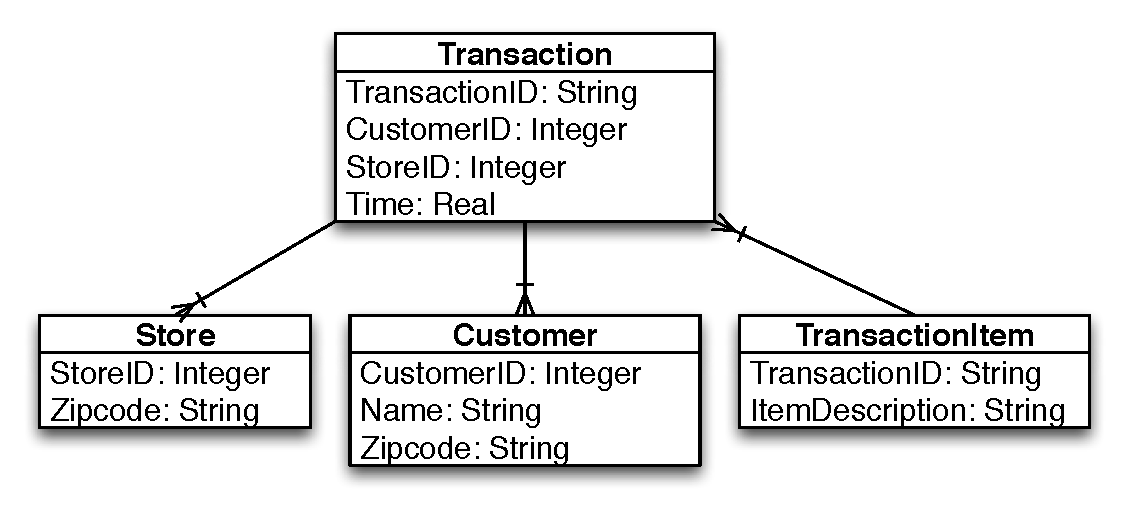
\includegraphics[width=3.5in]{figures/transactions_data_model.eps}
  \caption{Relational Data Model for Generated Data}
  \label{fig:relational-data-model}
\end{figure}


\subsection{Stores}
Store records consist of unqiue integer identifiers and locations given as zip codes.  The stores' zip codes are sampled from a probability mass function (PMF) where probabilities are linearly proportional to the zip code's population and exponentialy proportional to the zip code's median household income. The population and household income data for the zip codes were taken from from the U.S. Census American Community Survey \cite{ACS}.

\subsection{Customers}
Customer records consist of uniquer integer identifers, first names, last names, and locations given as zipcodes.  Names are generated using data from the Name Database\cite{NameDB}. Each record in the database gives a name, a weight, and flag indicatings if the name can be used as a first name, a last name, or both.  PMFs generated for the first and last names using the weights.  The customer's name is generated by sampling a first name and a last name from each PMF respectively.  Zip codes are sampled from a PMF where the probabilities are exponentially distributed according to the distance (in miles) to the nearest store's location. Distances are calculated using latitude and longitude coordinates taken from the Zip Code Database Project \cite{Zips}).

\subsection{Transactions}
Transactions records consist of customer, transaction, and store identifiers, the date and time of the transaction (as a real number indicating the number of days since the start of the simulation), and a list of purchased products. The customer and transaction identifiers form a unique composite key for each transaction record.

Transactions are simulated individually for each customer.  Transaction times are sampled using a Monte Carlo process.  Transaction times are proposed by sampling offsets before the exhaustion of products from an exponential distribution, with the average time parameterized separately for each customer by sampling from a uniform interval.  Acceptance probabilities are given by a separate PDF which can be used to model the effect of with factors such as store hours and customer work schedules.  Currently, the acceptance PDF only ensures that a new transaction time occurs after the previous transaction.  The proposed transaction time is accepted if a random number sampled uniformally from $[0, 1)$ is less than the acceptance probability. Otherwise, a new transaction time is proposed.

Product purchases are simulated by a separate process.  First, a state is chosen from the set of product categories and a stop state which indicates the end of the transaction.  Each product category's weight is exponentially proportional to the elapsed time between the transaction and exhaustion of the product category. The weight of the stop state is given by a constant which is zero until the first product is chosen.

Once a product category has been chosen, the process of choosing a product within the category is modelled by a Markov Model.  \textcolor{red}{The transition probabilites are determined by ...}. A product is chosen by advancing the state of the model by simulate one transition.  The state of the Markov Model is preserved between transactions.

Once a product has been chosen, the customer's inventory is updated and the exhaustion time is determined by simulating the usage of the products by numerically integrating a stochastic differential equation (SDE).  The purchasing process is restarted, using the updated exhaustion time.  If the stop state is chosen, the next transaction is generated.

%\begin{figure}[!t]
%  \centering
%  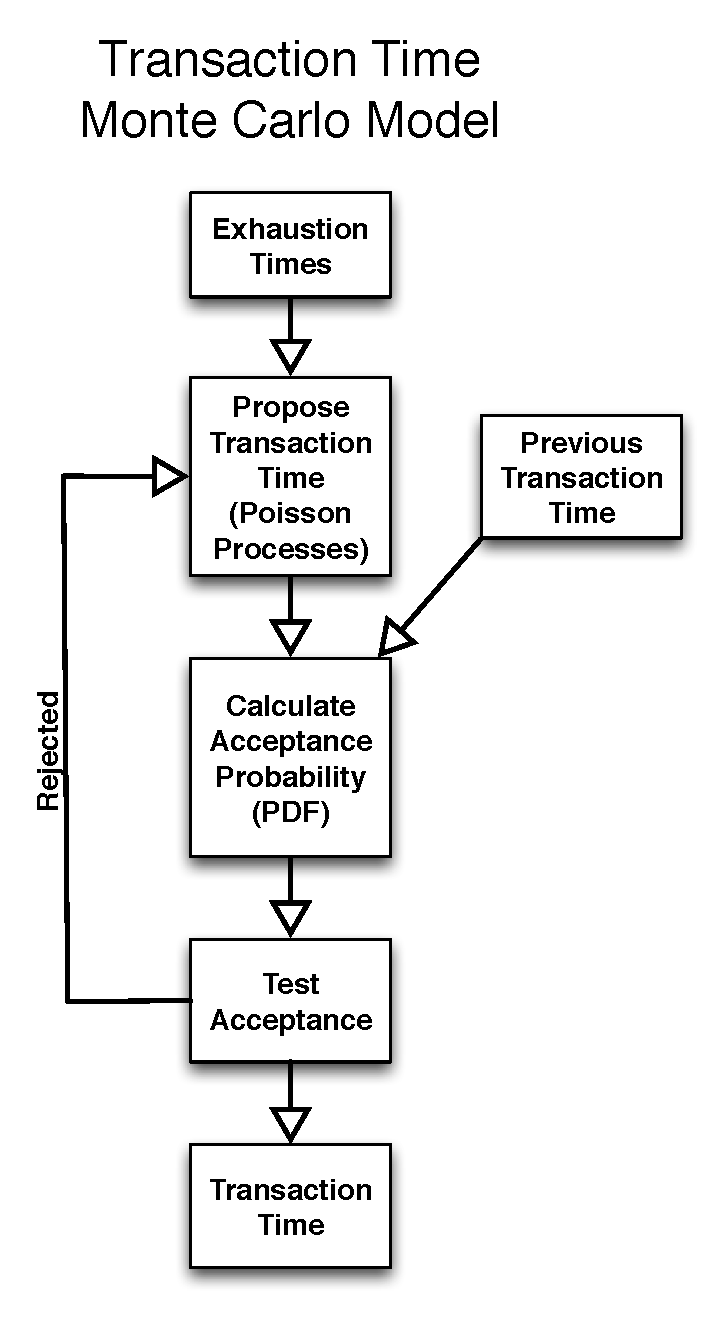
\includegraphics[width=3.5in]{figures/transaction_time_model.eps}
%  \caption{Transaction Time Monte Carlo Simulation}
%  \label{fig:trans_time}
%\end{figure}

%\begin{figure}[!t]
%  \centering
%  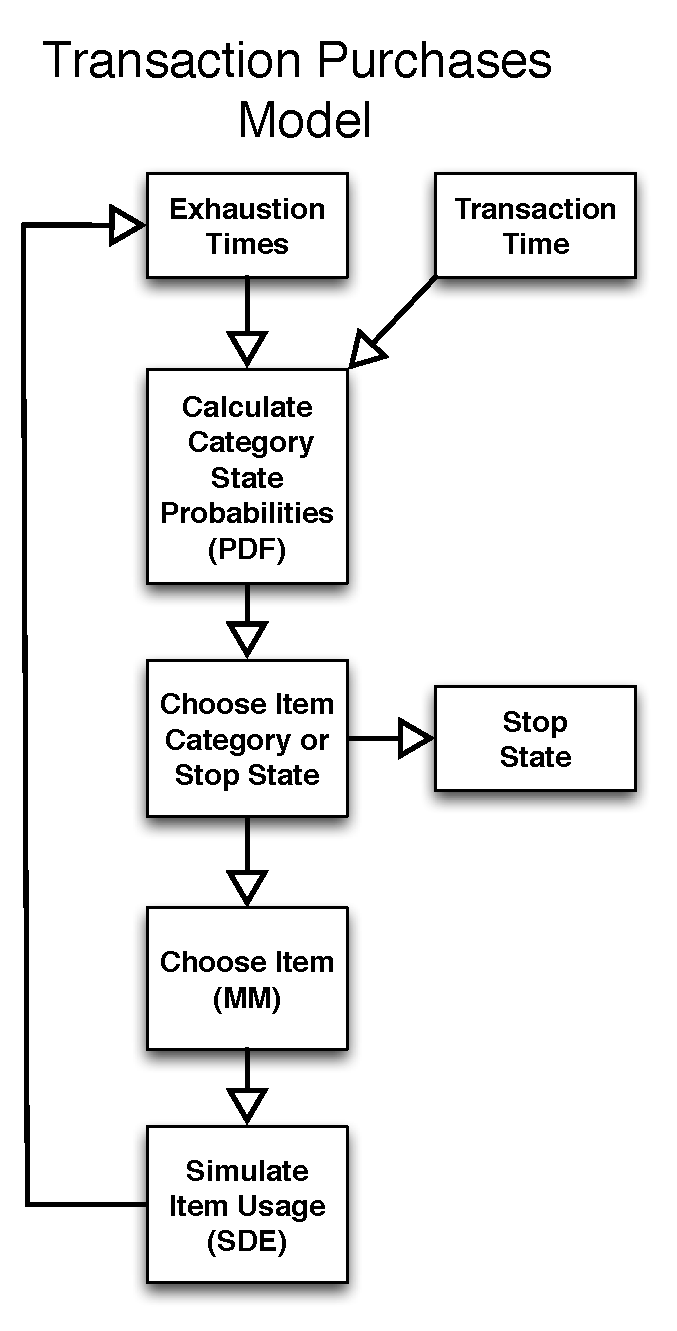
\includegraphics[width=3.5in]{figures/transaction_purchases_model.eps}
%  \caption{Transaction Purchases Monte Carlo Simulation}
%  \label{fig:purchases_sim}
%\end{figure}

%\begin{figure}[!t]
%  \centering
%  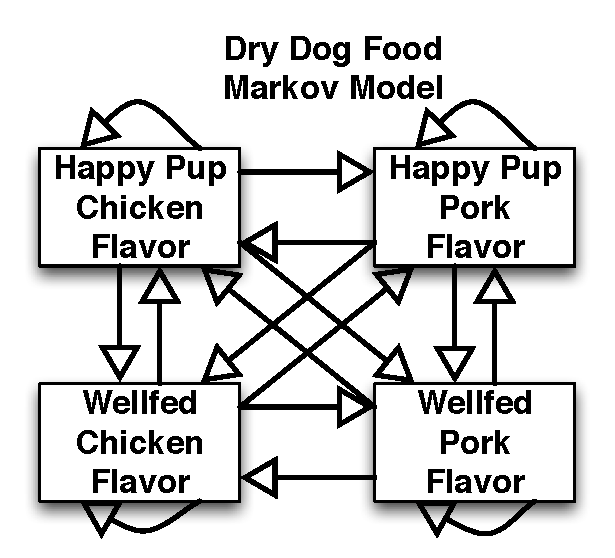
\includegraphics[width=3in]{figures/dog_food_markov_model.eps}
%  \caption{Example Markov Model for Dog Food}
%  \label{fig:dog_food_markov_model}
%\end{figure}

%\begin{figure}[!t]
%  \centering
%  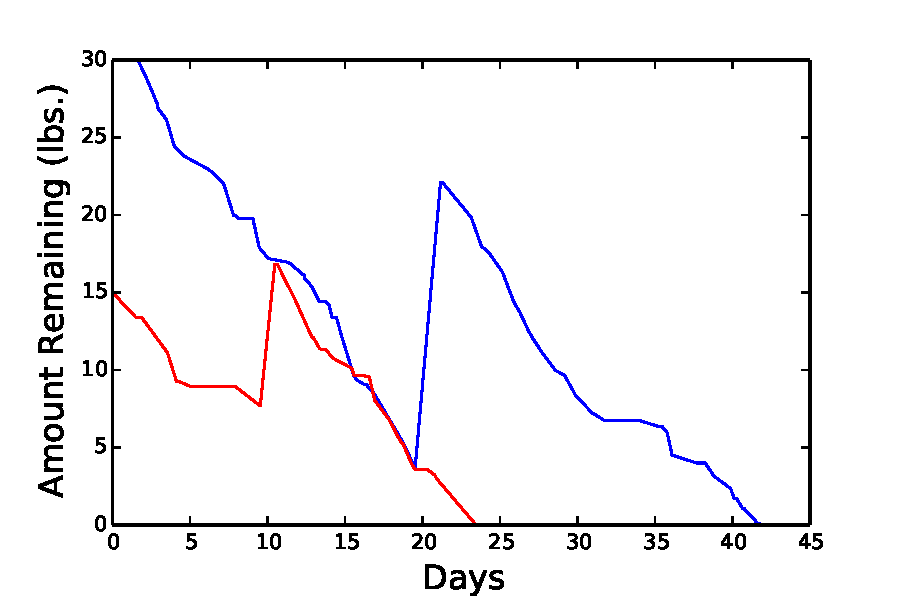
\includegraphics[width=3.5in]{figures/item_usage_simulation.pdf}
%  \caption{Example Product Usage Simulation}
%  \label{fig:product_usage_sim}
%\end{figure}


\section{Improvements to the Data Generator}
%\subsection{Products}
%The original data generator relied on a hand-generated JSON document containing product descriptions.  Due to the labor requirements, only a handful of products were available in each category with only 3-4 fields per category. To increase the number and variety of purchasing patterns in the model, a product enumerator was implemented.  Given a set of fields and possible values, the enumerator generates all combinations of products.

%Rules are used to filter out unwanted combinations of field values.  For example, the fictional brand of dog food ``Chef Corgi'' might be targeted towards budget-oriented consumers.  As such, the brands' products might exclude expensive ingredients and marketing (salmon, organic ingredients, etc.).  Products that do not satisfy the filters are removed from the list of possible products.

%Using the product enumerator, the number of products across four categories has been increased from \textcolor{red}{40 to over 3,000, and the number of fields has increased from 3-4 to upwards of 10 per category}.

%Optional products were introduced.  Examples of optional products include snacks, collars, sweaters, and toys. Exhaustion of optional products does not trigger transactions.  Said another way, the optional products' exhaustion times are not used when proposing transaction times.  There is no distinction between optional and mandatory products when simulating purchases within a transacton.

%\textcolor{red}{weather-triggered or seasonal products. product PDFs?}

\subsection{Association of Customers and Transactions with Stores}
In the data generator prototype, the store for each each transaction was picked uniformally from the set of all stores.  To improve upon the realism and support the incorporation of geospatial patterns, each customer is now associated with a specific store and all of a customer's transactions occur at that store.

In the new model, a store is sampled for each customer from a PMF with weights proportionally to population of the stores' zip codes.  The customers' locations are sampled from a PMF exponentially-distributed weights for each zip code $z$ according to the distance between the zip code $s$ of the customers' associated store:

\begin{equation}
w(s, z) = \lambda \exp(-\lambda d(s, z))
\end{equation}

where $\lambda$ is the inverse of the desired average distance.

\subsection{Weather Model}

\textcolor{red}{TODO why?}

Weather data is generated using a local weather model -- i.e., weather is not explicitly correlated between regions -- so that each region can be simulated independently for computational efficiency.  The model was derived and evaluated by comparing to local weather data downloaded from the NOAA QCLCD \textcolor{red}{cite}.  The goal of the model was not to accurately predict day-to-day weather patterns but to reproduce temporal and static statistical properties.  The model is similar in concept to other models \cite{Racsko1991,Chen2010,Birt2010,Fatichi2011} available in the literature.

Models were derived for daily average temperatures ($T(t)$, $^\circ$F), daily total precipitation ($P(t)$, in), and daily average wind speed ($V(t)$, mph). The temperature for each location is modeled as a first-order Fourier series plus noise generated by an Ornstein-Uhlenbeck process $Z(t)$ \cite{Gardiner09}:

\begin{align}
&T(t) = a_0 + a_1\sin\Big(\frac{-2 \pi t}{365}\Big) + a_2\cos\Big(\frac{-2 \pi t}{365}\Big) + Z(t) \\
&dZ(t) = - \gamma Z(t) dt + \sigma dW_t
\end{align}

The stochastic differential equation (SDE) for the Ornstein-Uhlenbeck process is integrated numerically using the Euler-Maruyama method \cite{Klouden13}:

\begin{align}
&Z_{t+1} = -\gamma Z_t \Delta t + \sigma \sqrt{\Delta t} \Delta W_{t+1} \\
&Z_0 = 0 \nonumber
\end{align}

The daily total precipitation for each region is assumed to be independently distributed from day-to-day and sampled from an exponential distribution:

\begin{equation}
P(t) \sim Exp(\lambda)
\end{equation}

where $\lambda$ is inverse of the daily average precipitation.

The daily average wind speed for each region is modeled using a first-order Fourier series and values sampled independently day-to-day from an Erlang distribution:

\begin{align}
&V(t) = b_0 + b_1\sin\Big(\frac{-2 \pi t}{365}\Big) + b_2\cos\Big(\frac{-2 \pi t}{365}\Big) + X(t) \\
&X(t) \sim Erlang(k, \theta)
\end{align}

where $k$ and $\theta$ are the shape and scale parameters, respectively.

From the temperature, precipitation and wind speed, the snowfall ($S(t)$, in), rainfall ($R(T)$, in), and wind chill ($WC(T)$, $^\circ$F) \textcolor{red}{cite} are calculated as follows:

\begin{align}
&r(t) = \frac{1}{1 + \exp(-a (T - b))} \\
&S(t) = 10 (1 - r(t)) P(T) \\
&R(T) = r(t) P(T)
\end{align}

\begin{align}
WC(T) = 35.74 + &0.6215T(t) - 35.75V^{0.16}(t) \, + \\ \nonumber
&0.4275T(t)V^{0.16}(t)
\end{align}

Model parameters were estimated separately for each weather station in the NOAA QCLCD data from October 2011 to September 2014.  Weather stations missing more than 5\% of the data were excluded.  The Fourier coefficients $a_0$, $a_1$, $a_2$, $b_0$, $b_1$, and $b_2$ were found from Fourier transforms of the daily average temperature and daily average wind speed data. The distribution parameters $\sigma$, $\lambda$, $k$, and $\theta$ were computed directly from the data using the Maximum Likelihood Estimaters (MLE).  The damping coefficient $\gamma$ was determined empirically and the same value was used for every weather station.

Local weather simulations are run for each store using model parameters from the closest weather stations. The closest weather station is found for each store by computing the distances from the GPS coordinates of the stores' zip codes and weather station from the NOAA QCLCD data. 

\subsection{Incorporating the Effect of Weather on Transaction Times}
The transaction time model was updated to incorporate the effect of the daily weather on customers' shopping times.

Separate conditional probability density functions (PDFs) giving the probability of a transaction occuring on day $d_i$ is given for the daily wind chill and snow fall.  The PDFs are modeled using sigmoidal functions:

\begin{equation}
P(\text{trans}_{d_i}=\text{YES}|x_{d_i}) = \frac{A}{1+\exp(-B(x-C))}+D
\end{equation}

\textcolor{red}{TODO table of parameters}

The probability of a transaction occurring on a day $d_i$ is given by the minimum probability of the individual PDFs:

\begin{align}
P(\text{trans}_{d_i}=\text{YES} | S_{d_i}, WC_{d_i}) = &\min \, \{ P(\text{trans}_{d_i}=\text{YES}|S_{d_i}), \nonumber \\ 
&P(\text{trans}_{d_i}=\text{YES} | WC_{d_i}) \, \}
\end{align}

The transaction time model was modified by adding the weather PDF to the transaction time acceptance probability PDF for transaction time $t_i$:

\begin{align}
P(\text{trans}_{t_i}&=\text{YES}|t_{i-1}, S_{d_i}, WC_{d_i}) = \nonumber \\
&Z^{-1} P(\text{trans}_{t_i}=\text{YES}|t_{i-1}) P(\text{trans}_{d_i}=\text{YES} | S_{d_i}, WC_{d_i})
\end{align}
 
where $Z$ is the normalization factor.  



\subsection{Java Library Implementation}
The data generator was originally prototyped in Python \cite{Nowling14}.  Once the utility of the generator was validated, the generator was implemented as a Java library for production usage. Java was chosen for compatibility with popular big data processing systems such as Apache Hadoop \cite{Hadoop} and Apache Spark \cite{Zaharia2010,Zaharia2012} and other JVM languages such as Scala and Clojure.  The Java implementation has ~5,500 lines of code, ~110 classes, and ~90 unit tests.

The library's API is relatively simple with one class for loading input data, five classes for generating data, and six data model classes.  Broad support for multiple parallelization paradigms was a primary design requirement.  Generators interact only through standard Java collections containing serializable objects and are designed to allow multiple instantiated copies to support parallelization.  As such, parallelization is as simple as creating as many independent instances as needed and combining the resulting Java collections before each stage. An example driver implemented with Apache Spark with support for parallel and distributed computing is presented in Section~\ref{sec:spark}.  For development purposes, the library includes a single-threaded command-line driver.

\begin{figure}[!t]
  \centering
  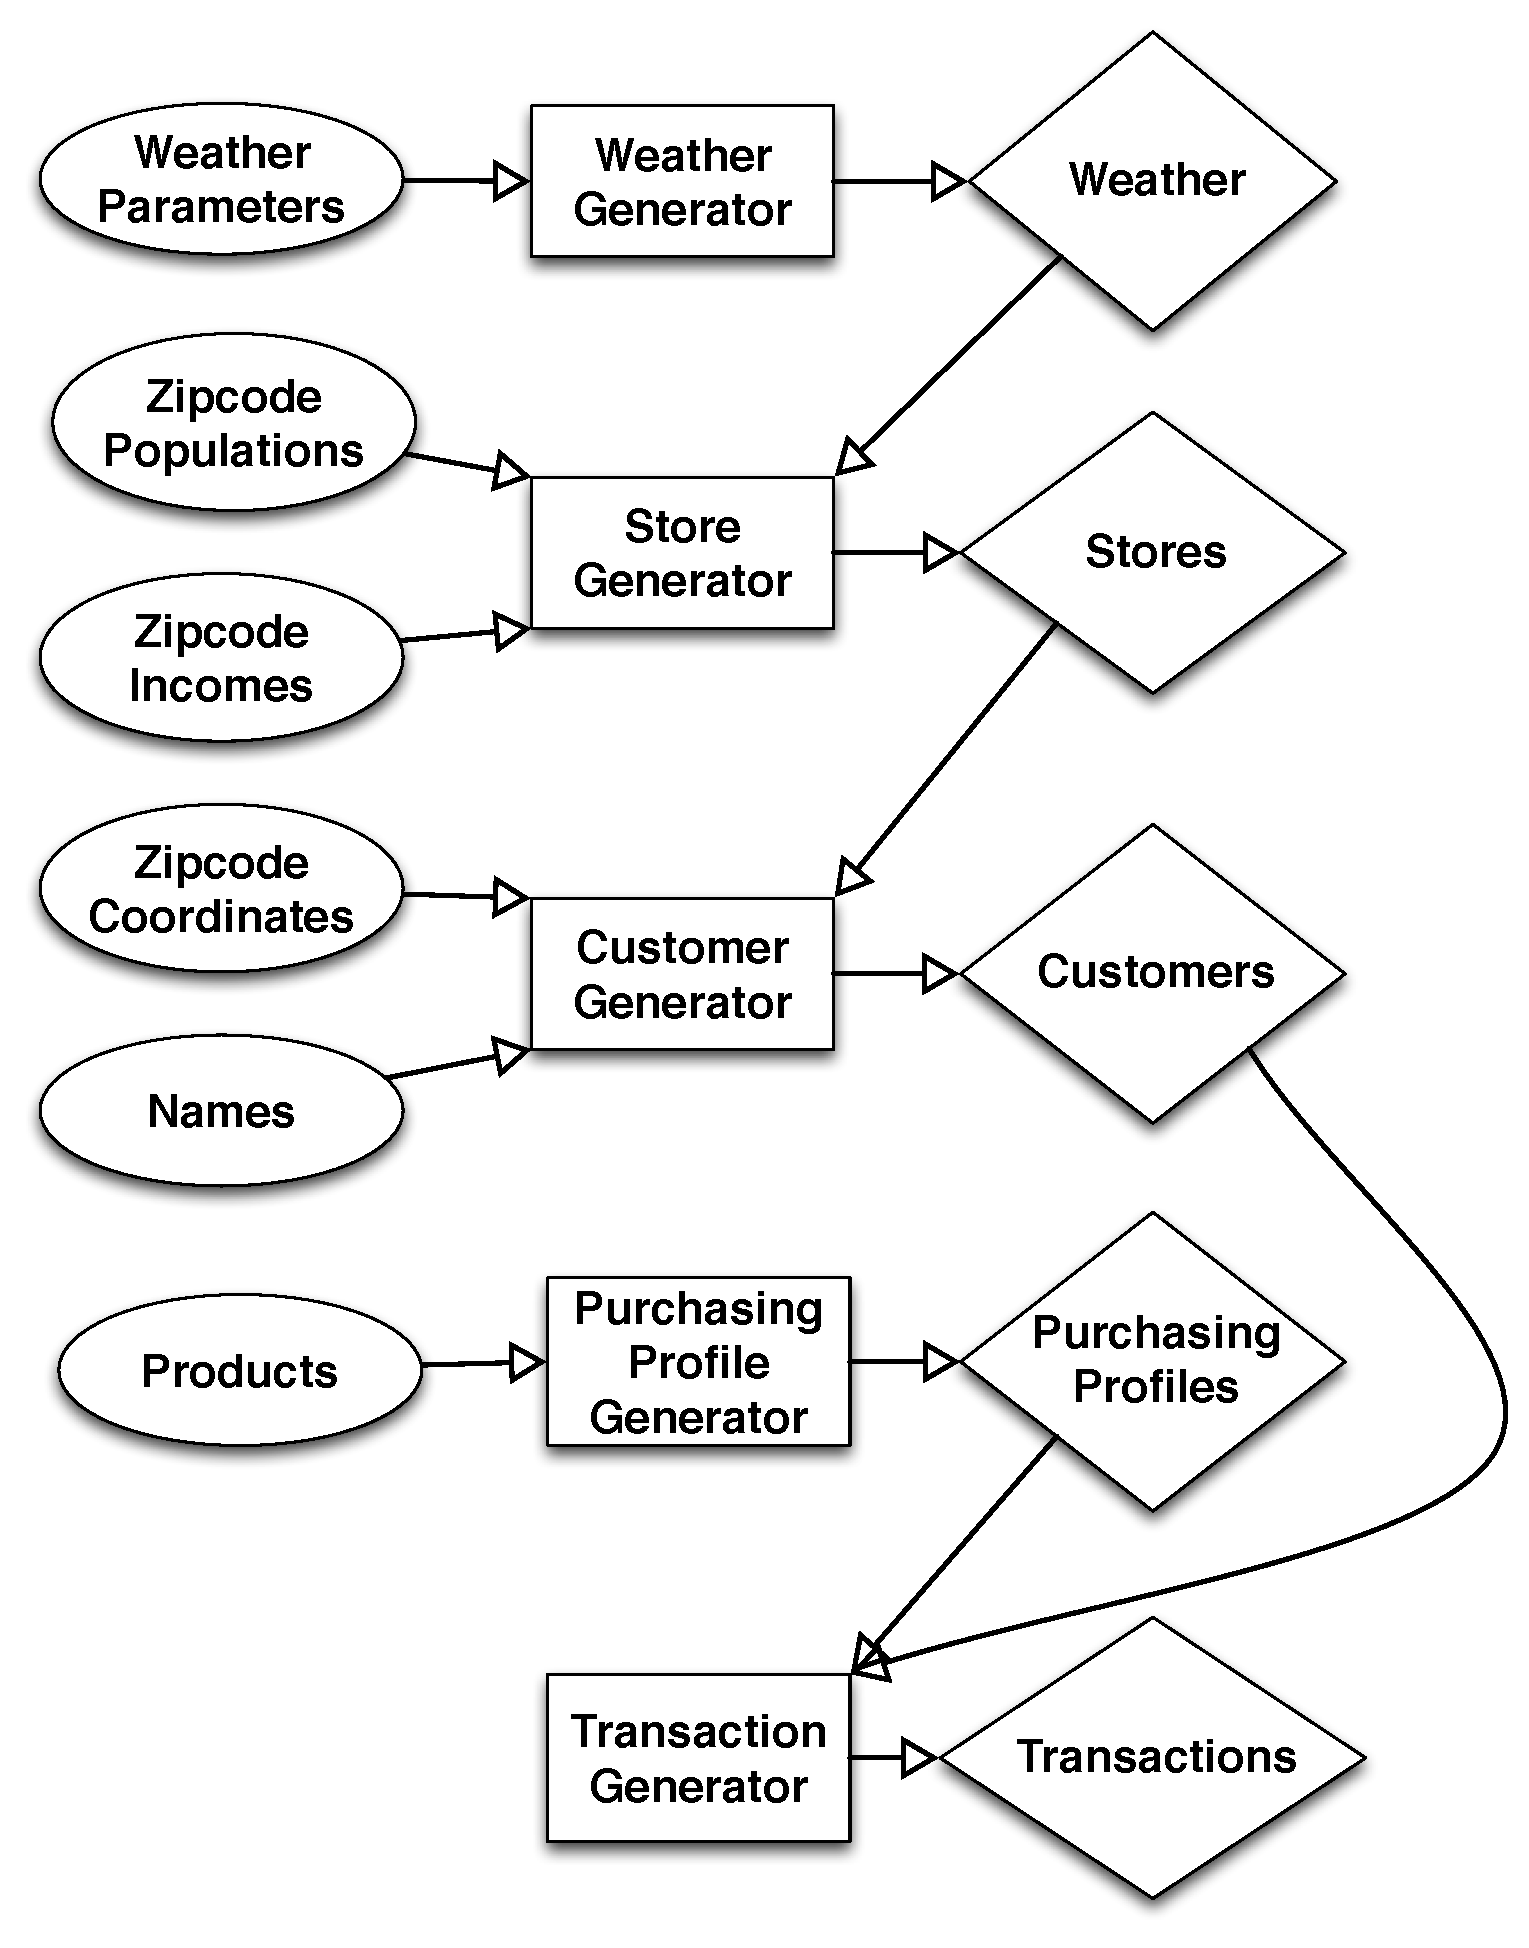
\includegraphics[width=3.5in]{figures/bps_flowchart.eps}
  \caption{BigPetStore Flowchart. Ovals represent input data, rectangles represent data generators, and diamonds represent generated data.}
  \label{fig:bps_flowchart}
\end{figure}

The source code is available at \url{https://github.com/rnowling/bigpetstore-data-generator} under the Apache Public License v2. Jars are published via \textcolor{red}{\url{bintray}} for easy integration with build systems that support automatic dependency resolution.  

\section{Parallelization with Spark Driver} \label{sec:spark}
\textcolor{red}{TODO code listing}

\section{Evaluation of the Model}
To evaluate the changes in the model, we analyzed data for 10 stores, 10,000 customers, and five years of transactions generated from the model. 

\subsection{Comparison of Real and Simulated Weather Data}
Three years of observed daily average temperature, total precipitation, and average wind speed from the NOAA QCLCD data \textcolor{red}{cite} for South Bend, IN from October 2011 to September 2014 are shown in Figure~\ref{fig:weather-model} alongside simulated data generated from the model. The simulated data is able to produce temporal and stationary patterns similar to those of the real data.


\begin{figure*}[!t]
  \centering
  \begin{subfigure}[b]{0.4\textwidth}
    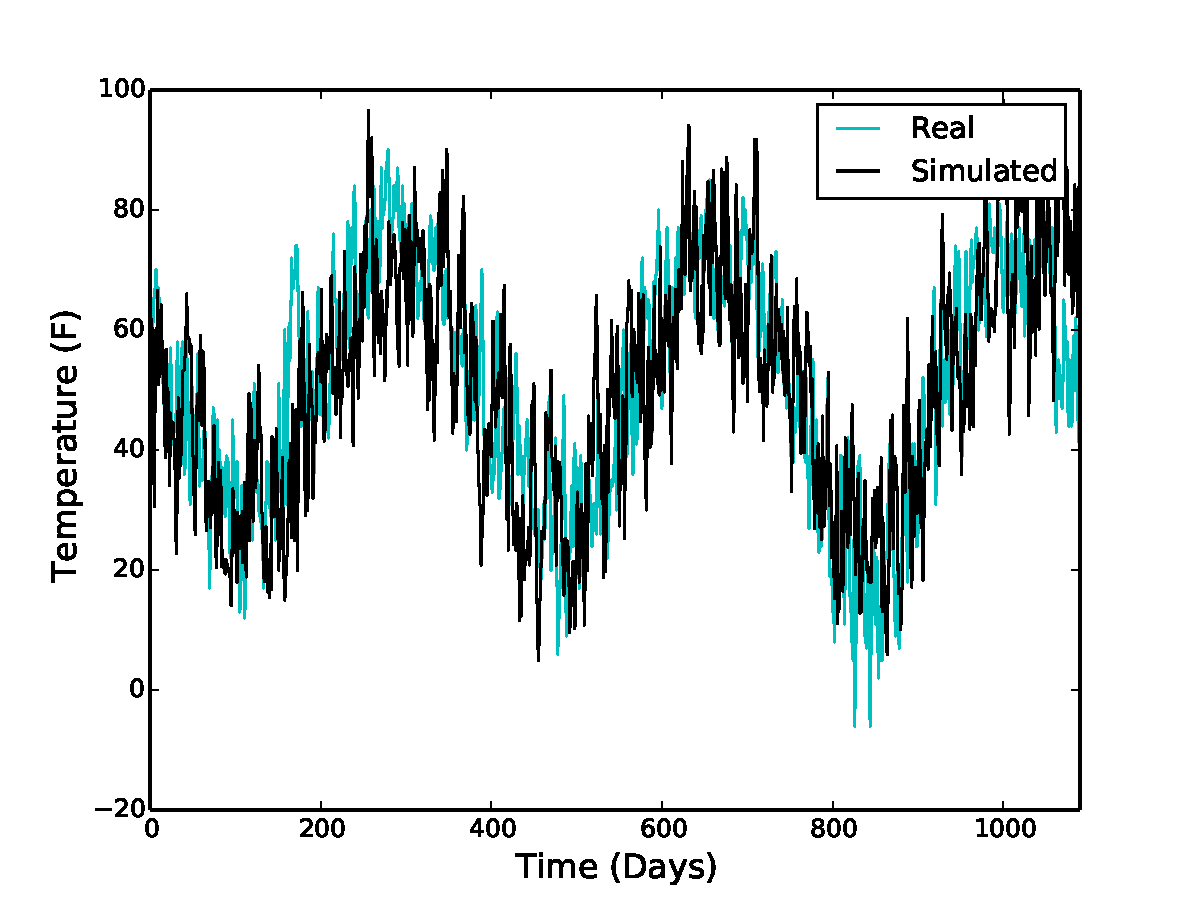
\includegraphics[width=\textwidth]{figures/sim_temp.pdf}
    \caption{Daily Temperature}
  \end{subfigure}
  ~
  \begin{subfigure}[b]{0.4\textwidth}
    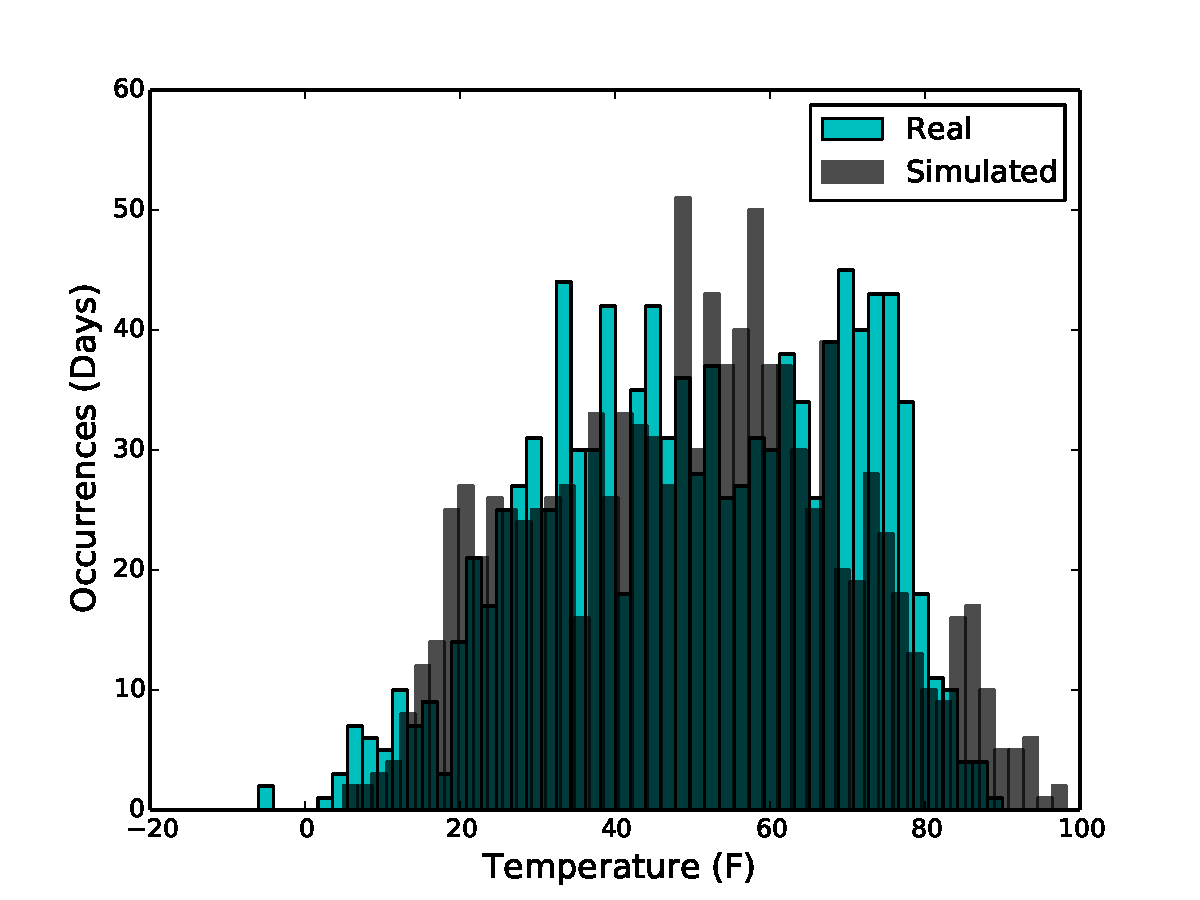
\includegraphics[width=\textwidth]{figures/sim_temp_hist.pdf}
    \caption{Temperature Histogram}
  \end{subfigure}
  ~
  \begin{subfigure}[b]{0.4\textwidth}
    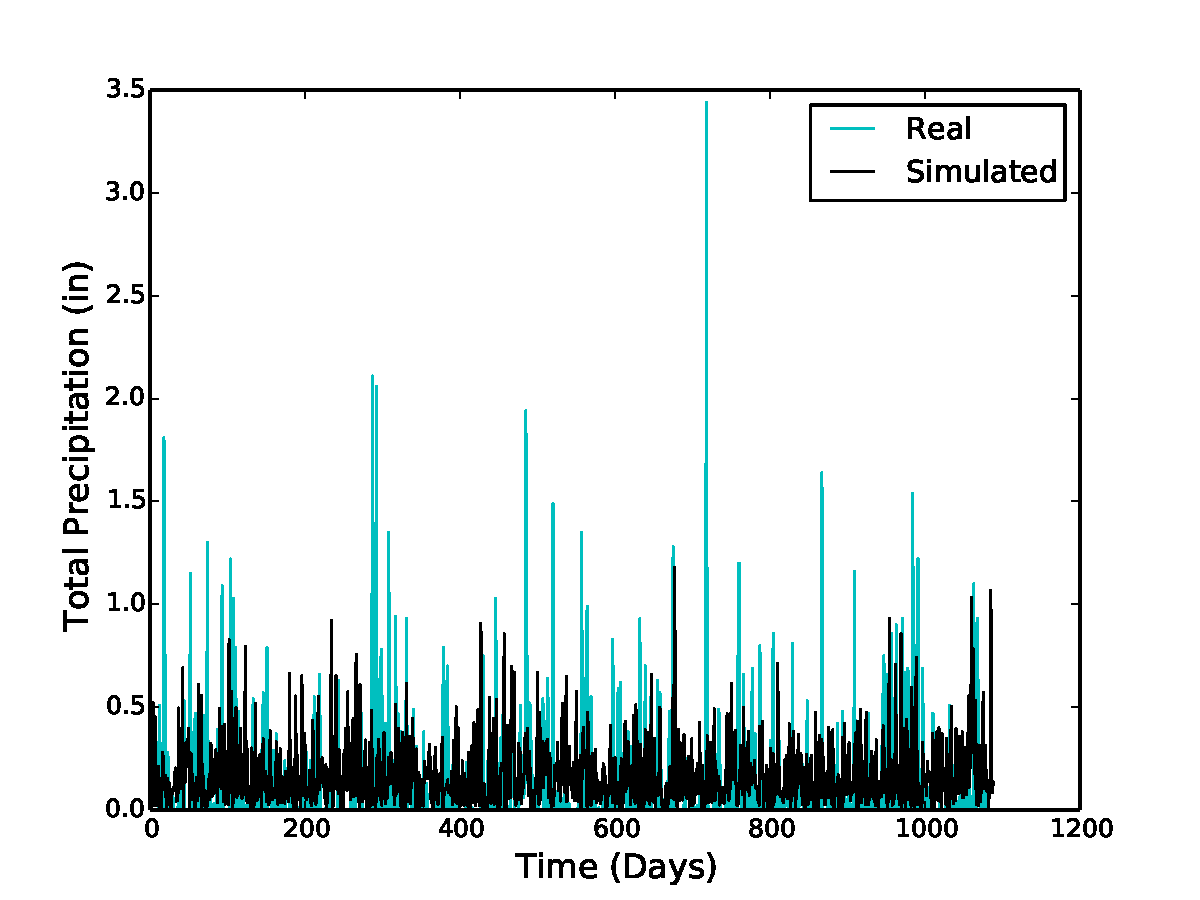
\includegraphics[width=\textwidth]{figures/daily_precip.pdf}
    \caption{Daily Precipitation}
  \end{subfigure}
  ~
  \begin{subfigure}[b]{0.4\textwidth}
    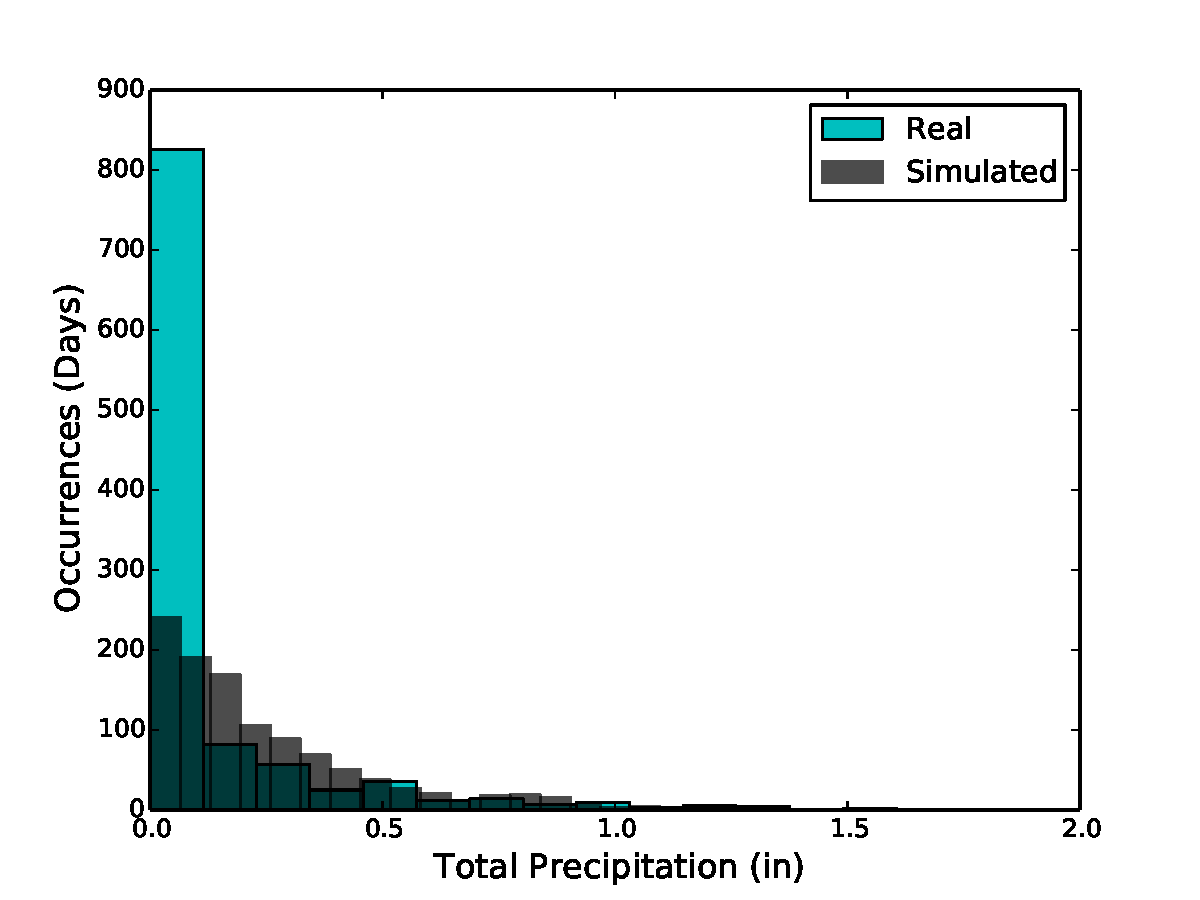
\includegraphics[width=\textwidth]{figures/daily_precip_hist.pdf}
    \caption{Precipitation Histogram}
  \end{subfigure}
  ~
  \begin{subfigure}[b]{0.4\textwidth}
    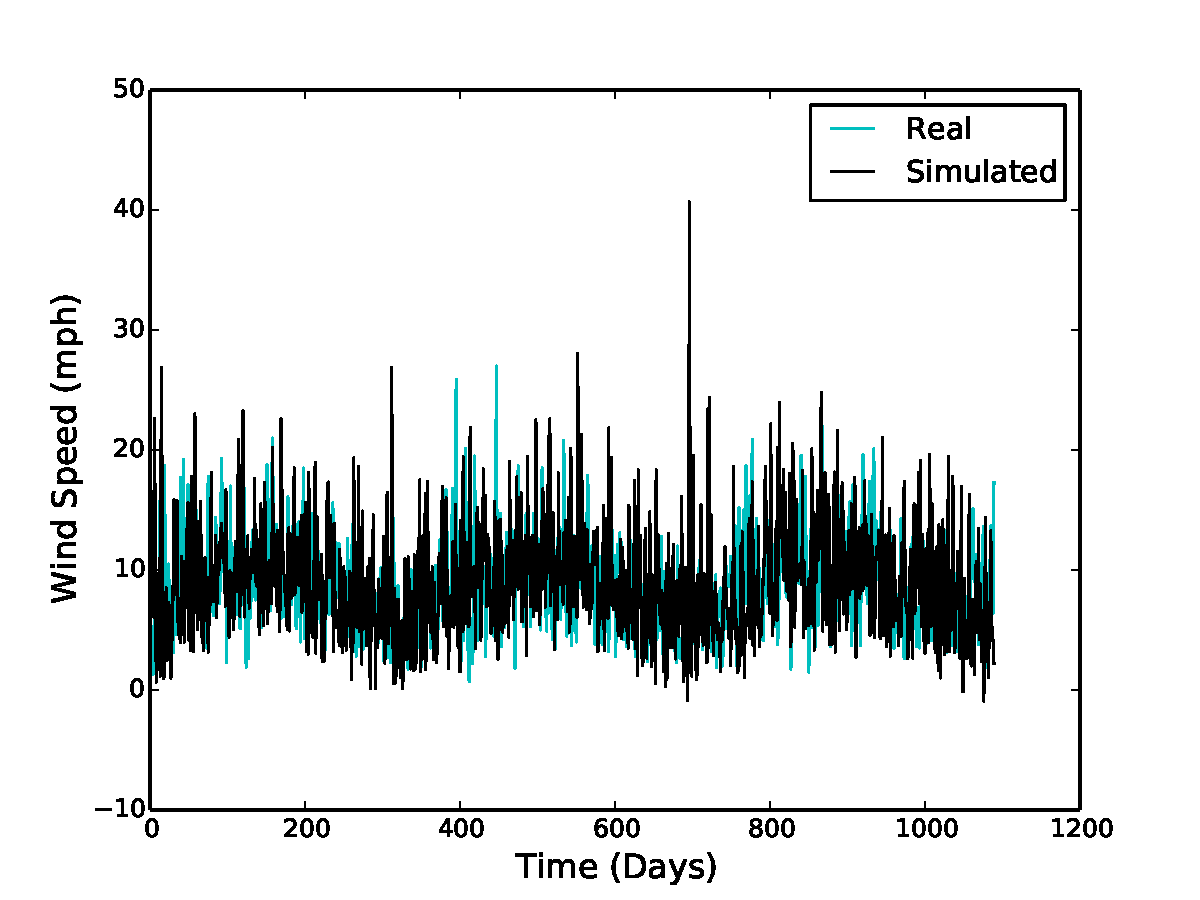
\includegraphics[width=\textwidth]{figures/daily_wind_speeds.pdf}
    \caption{Daily Wind Speed}
  \end{subfigure}
  ~
  \begin{subfigure}[b]{0.4\textwidth}
    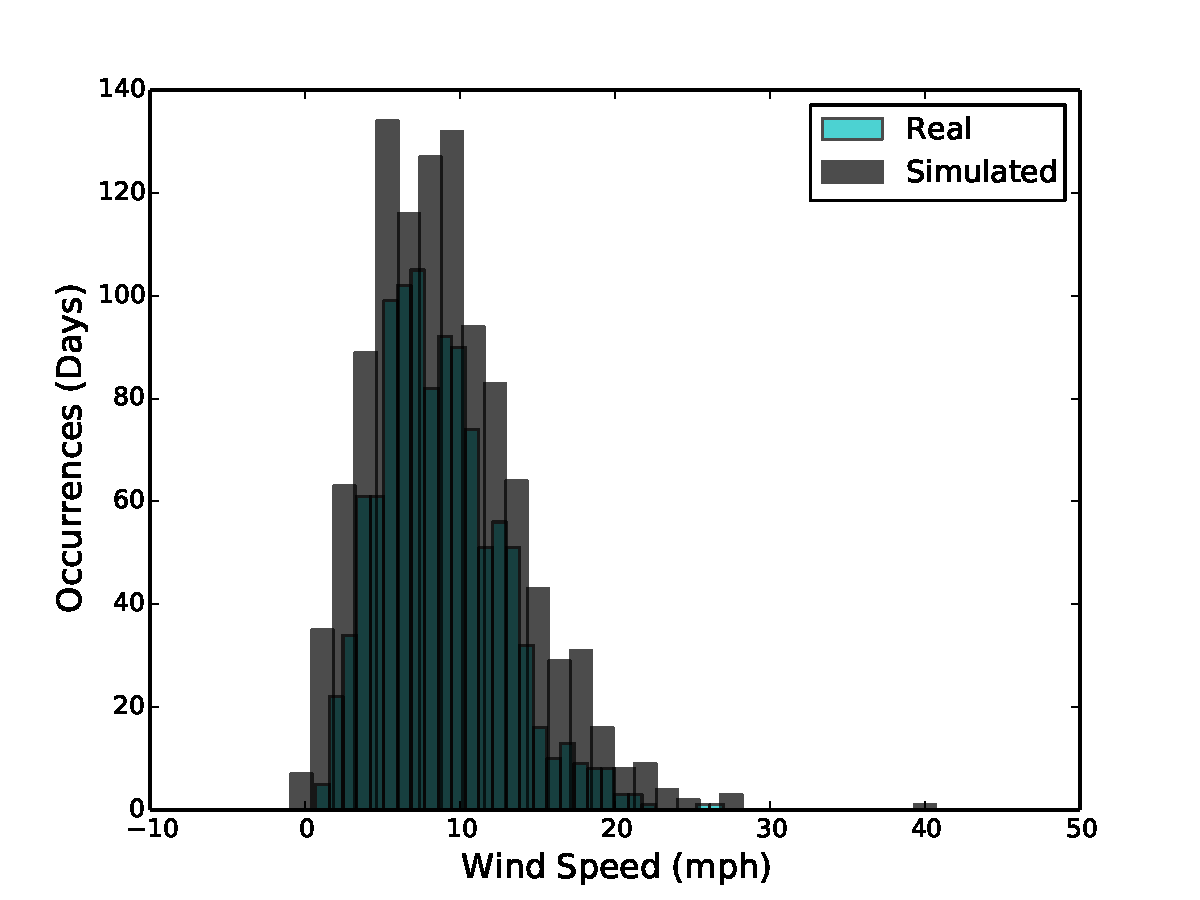
\includegraphics[width=\textwidth]{figures/daily_wind_speed_hist.pdf}
    \caption{Wind Speed Histogram}
  \end{subfigure}

  \caption{NOAA QCLCD weather data alongside simulated data for South Bend, IN for October 2011 to September 2014.}
  \label{fig:weather-model}  
\end{figure*}

\subsection{Weekly Transaction Counts by Store}
The weekly transaction counts over five years of simulation for six stores are plotted in Figure~\ref{fig:weekly-trans-counts}.  The variation in the number of transactions by store validates that the model is assigning customers to stores in proportion to the population of the stores' zip codes.  Large fluctuations in the weekly transaction counts occur during winter months, validating that the weather transaction model is capturing the effect of weather on transaction times.

\begin{figure}[!h]
  \centering
  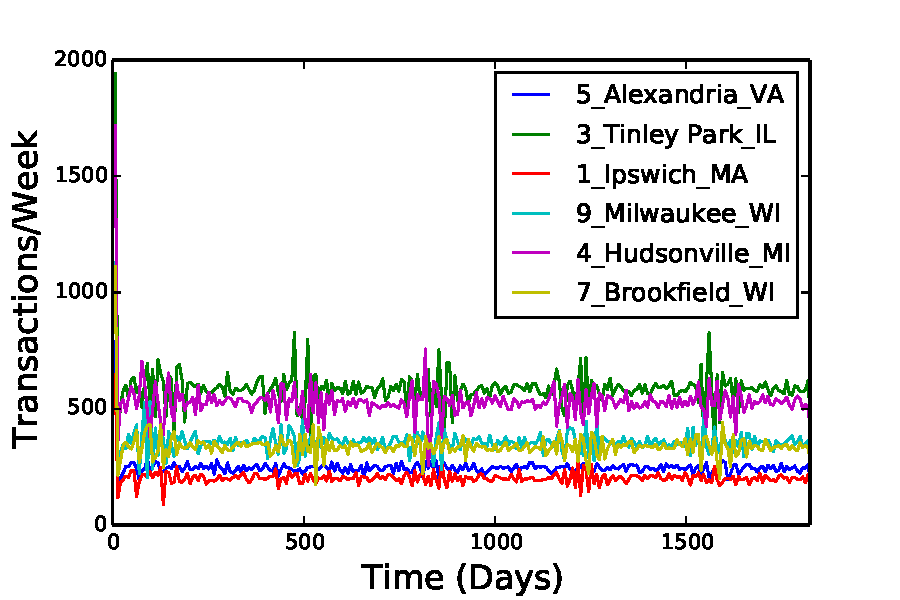
\includegraphics[width=3.5in]{figures/weather_weekly_transaction_counts.pdf}
  \caption{Stores' Weekly Transaction Counts}
  \label{fig:weekly-trans-counts}
\end{figure}

\subsection{Impact of Weather on Shopping Patterns by Region}

\textcolor{red}{TODO: effect of weather, variations by region}

%\subsection{Customer Segmentation}
%Secondly, we profiled our customers' purchasing habits to optimize the advertising campaign's effectiveness by customizing the advertised products for each customer.  For each customer, we generated a feature vector by computing the frequency with which they would purchase the same brand or flavor from one transaction to the next.  We clustered the customers' feature vectors using the KMeans algorithm with a range of cluster counts. Twenty clusters converged the error.

%\begin{figure}[!t]
%  \centering
%  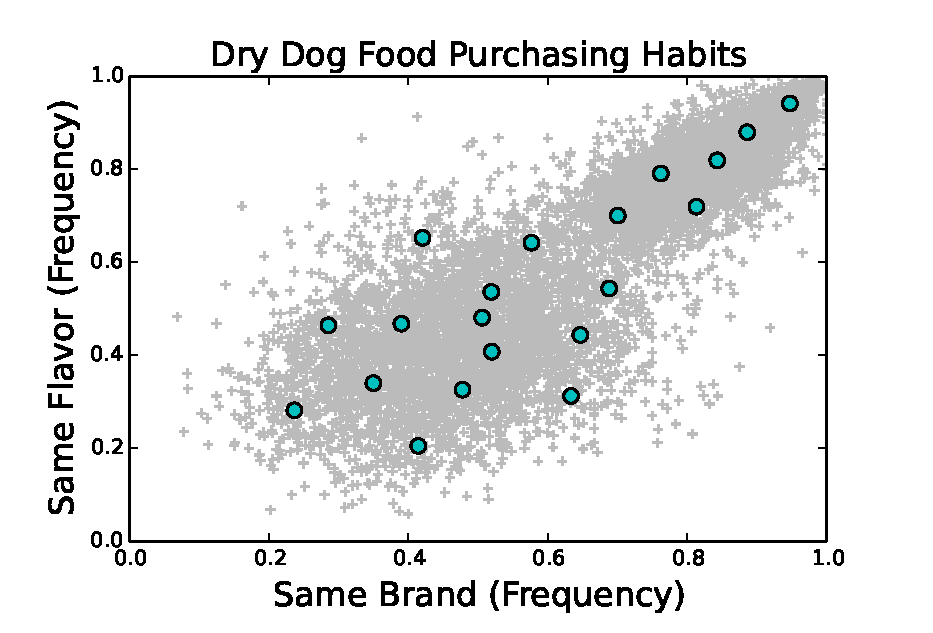
\includegraphics[width=3.5in]{figures/cluster_analysis.eps}
%  \caption{Clustering of Brand and Flavor Purchasing Preferences. Grey plus signs (+) represent customer data points, and cyan circles represent cluster centers.}
%  \label{fig:cluster_analysis}
%\end{figure}

%Analysis of the feature vectors and clusters revealed four predominant purchasing profiles (Figure~\ref{fig:cluster_analysis}).  High frequencies of purchasing the same flavors repeatedly were tightly-correlated with high frequencies of purchasing the same brands -- these customers were likely to be happy with a particular item and kept purchasing the same item repeatedly.  For our advertising campaign, it would be unlikely to get these customers to purchase different items, so we should create incentives to purchase larger quantities, especially when inventory levels are high and needed to be depleted.  Other customers had a tendency to purchase either the same flavor or brand repeatedly, but varied in their choice of the other.  For customers who prefer a particular brand, we should target our advertising campaign to suggest other flavors sold by that brand.  Likewise, for customers who prefer a particular flavor, we should target our advertising campaign to suggest other brands with that flavor.  Lastly, some customers had very low frequencies of purchasing neither the same brand nor flavor.  Other factors, such as cost, not represented in this analysis may be driving these customers' purchasing habits and will need further study.

%\textcolor{red}{compare new and old}

\section{Discussion and Conclusion}
The BigPetStore data generator is a domain-driven mathematical model and simulation for generating data with rich patterns.  A new model for local weather simulation which enabled the incorporation of additional geospatial and temporal correlations was described. A new JVM library implementation was described.  Support for parallelization and interopability with tools in the big data ecosystem was demonstrated using an Apache Spark driver.

\textcolor{red}{The math model was validated using ...}

We see multiple opportunities for building on the work presented.  \textcolor{red}{...}

We intend to expand the model to incorporate additional factors.  Deeper integration of existing fields such as location and purchasing profiles (e.g., to model regional purchasing preferences) will increase the variety of the semantic information encoded in the generated data. The incorporation of weather and climate data can be used to influence when customers shop, the types of products they buy, and the amount of products purchased. For example, customers would be less likely to shop during snow storms, more likely to buy items such as winter apparel for their pets, and more likely to purchase bulk quantities to reduce the number of transactions. Modeling of time-dependent events such as sales, evolution of customer purchasing profiles over time, and ``life events,'' such as the birth or passing of pets, will enable more interesting time-series analysis of the data.  We would also like to expand the scope of the model to incorporate business processes (such as inventory management, customer complaints, employees, etc.), thus enabling queries about the relationship between internal business process and customer behavior.


% no \IEEEPARstart
%This demo file is intended to serve as a ``starter file''
%for IEEE conference papers produced under \LaTeX\ using
%IEEEtran.cls version 1.7 and later.
% You must have at least 2 lines in the paragraph with the drop letter
% (should never be an issue)
%I wish you the best of success.

%\hfill mds
 
%\hfill January 11, 2007


% An example of a floating figure using the graphicx package.
% Note that \label must occur AFTER (or within) \caption.
% For figures, \caption should occur after the \includegraphics.
% Note that IEEEtran v1.7 and later has special internal code that
% is designed to preserve the operation of \label within \caption
% even when the captionsoff option is in effect. However, because
% of issues like this, it may be the safest practice to put all your
% \label just after \caption rather than within \caption{}.
%
% Reminder: the "draftcls" or "draftclsnofoot", not "draft", class
% option should be used if it is desired that the figures are to be
% displayed while in draft mode.
%
%\begin{figure}[!t]
%\centering
%\includegraphics[width=2.5in]{myfigure}
% where an .eps filename suffix will be assumed under latex, 
% and a .pdf suffix will be assumed for pdflatex; or what has been declared
% via \DeclareGraphicsExtensions.
%\caption{Simulation Results}
%\label{fig_sim}
%\end{figure}

% Note that IEEE typically puts floats only at the top, even when this
% results in a large percentage of a column being occupied by floats.


% An example of a double column floating figure using two subfigures.
% (The subfig.sty package must be loaded for this to work.)
% The subfigure \label commands are set within each subfloat command, the
% \label for the overall figure must come after \caption.
% \hfil must be used as a separator to get equal spacing.
% The subfigure.sty package works much the same way, except \subfigure is
% used instead of \subfloat.
%
%\begin{figure*}[!t]
%\centerline{\subfloat[Case I]\includegraphics[width=2.5in]{subfigcase1}%
%\label{fig_first_case}}
%\hfil
%\subfloat[Case II]{\includegraphics[width=2.5in]{subfigcase2}%
%\label{fig_second_case}}}
%\caption{Simulation results}
%\label{fig_sim}
%\end{figure*}
%
% Note that often IEEE papers with subfigures do not employ subfigure
% captions (using the optional argument to \subfloat), but instead will
% reference/describe all of them (a), (b), etc., within the main caption.


% An example of a floating table. Note that, for IEEE style tables, the 
% \caption command should come BEFORE the table. Table text will default to
% \footnotesize as IEEE normally uses this smaller font for tables.
% The \label must come after \caption as always.
%
%\begin{table}[!t]
%% increase table row spacing, adjust to taste
%\renewcommand{\arraystretch}{1.3}
% if using array.sty, it might be a good idea to tweak the value of
% \extrarowheight as needed to properly center the text within the cells
%\caption{An Example of a Table}
%\label{table_example}
%\centering
%% Some packages, such as MDW tools, offer better commands for making tables
%% than the plain LaTeX2e tabular which is used here.
%\begin{tabular}{|c||c|}
%\hline
%One & Two\\
%\hline
%Three & Four\\
%\hline
%\end{tabular}
%\end{table}


% Note that IEEE does not put floats in the very first column - or typically
% anywhere on the first page for that matter. Also, in-text middle ("here")
% positioning is not used. Most IEEE journals/conferences use top floats
% exclusively. Note that, LaTeX2e, unlike IEEE journals/conferences, places
% footnotes above bottom floats. This can be corrected via the \fnbelowfloat
% command of the stfloats package.



% \section{Conclusion}
%The conclusion goes here.




% conference papers do not normally have an appendix


% use section* for acknowledgement
\section*{Acknowledgment}
The authors would like to thank Brian P. Clare and Casey Robinson for useful and interesting discussion.  Will Benton, Trevor M. Cickovski, Erik Erlandson, Scott A. Hale, Hank Jakiela, Casey Robinson, and Douglas Thain provided invaluable feedback on the manuscript.  JV would like to thank the Apache BigTop community for their interest in and support of BigPetStore.  The authors would also like to thank Matt Fenwick, Nigel Savage, and Bhashit Parikh for their contributions to BigPetStore. The authors would like to thank Red Hat, Inc. and the University of Notre Dame for their support of this work.





% trigger a \newpage just before the given reference
% number - used to balance the columns on the last page
% adjust value as needed - may need to be readjusted if
% the document is modified later
%\IEEEtriggeratref{8}
% The "triggered" command can be changed if desired:
%\IEEEtriggercmd{\enlargethispage{-5in}}

% references section

% can use a bibliography generated by BibTeX as a .bbl file
% BibTeX documentation can be easily obtained at:
% http://www.ctan.org/tex-archive/biblio/bibtex/contrib/doc/
% The IEEEtran BibTeX style support page is at:
% http://www.michaelshell.org/tex/ieeetran/bibtex/
\bibliographystyle{IEEEtran}
% argument is your BibTeX string definitions and bibliography database(s)
\bibliography{IEEEabrv,paper}
%\bibliography{paper}
%
% <OR> manually copy in the resultant .bbl file
% set second argument of \begin to the number of references
% (used to reserve space for the reference number labels box)
%\begin{thebibliography}{1}

%\bibitem{IEEEhowto:kopka}
%\subsection{Subsection Heading Here}
%Subsection text here.


%\subsubsection{Subsubsection Heading Here}
%Subsubsection text here.
%H.~Kopka and P.~W. Daly, \emph{A Guide to \LaTeX}, 3rd~ed.\hskip 1em plus
%  0.5em minus 0.4em\relax Harlow, England: Addison-Wesley, 1999.

%\end{thebibliography}




% that's all folks
\end{document}


